\section{Common Variations - Multiple Transactions}
\label{sec:buy_sell_stocks:multiple_transaction}

\subsection{Problem statement}
\begin{exercise}
    You are given an integer array $P$ where $P[i]$ contains the price of a given stock on the $i^{th}$ day.

    On each day, you may decide to buy and/or sell the stock. 
    You can only hold at most one share of the stock at any given time.
    However, you might engage in multiple transactions over the course of time i.e. you repeat the process of buying a share then selling it after a while (also the next day) multiple times.
    
    Write a function that given $P$ returns the maximum profit achievable.

    Notice that you may not engage in multiple transactions at the same time i.e., you must sell the stock before you buy it again.
    \begin{example}
    \label{ex:buy_sell_stocks_2:exmaple1}
        \hfill \\
        Given the array of prices for the stock is $[7,1,5,3,6,4]$, the answer is $7$. 
        You can buy on the \nth{2} day and sell on the \nth{3} and then engage on a second transaction where you buy on the \nth{4} day and sell on the \nth{5}.
    \end{example}

\end{exercise}


\section{Discussion}
\label{buy_sell_stocks_2:sec:discussion}
This might seems like an harder problem at first than the version presented in Section \ref{sec:buy_sell_stocks:statement1} but in reality as we will see in Section \ref{buy_sell_stocks_2:sec:linear} its solution is actually easier.

\section{Brute force solution}
\label{buy_sell_stocks_2:sec:bruteforce}
As usual, we start our discussion by quickly presenting the brute force solution. In this case, this means trying all possible sets of transactions (a valid pair of buying and selling operations not overlapping with any other transaction). We can try all possible sets by using recursion cleverly. However, this approach will not take us far because the number of possible sets of transactions grows exponentially.
We are showing this approach in Listing \ref{list:buy_sell_stocks_2:bruteforce}  only because we think its implementation can be somehow instructive.

\lstinputlisting[language=c++, caption={Bruteforce exponential solution to the problem of buying and selling stock with no limits on the number of transactions.},label=list:buy_sell_stocks_2:bruteforce]{sources/buy_sell_stocks/buy_sell_stocks_2/buy_sell_stocks_2_solution1.cpp}

\section{Linear time solution}
\label{buy_sell_stocks_2:sec:linear}
\begin{figure}
	\centering
	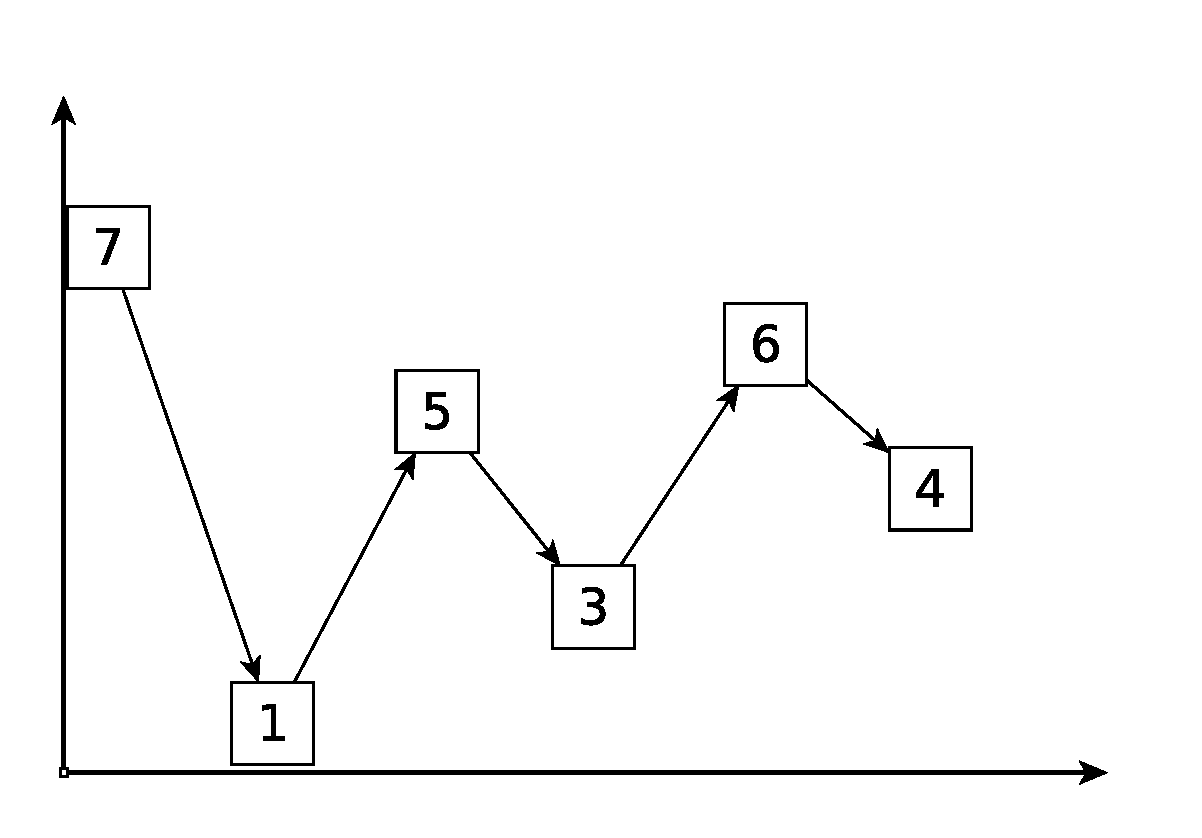
\includegraphics[width=\textwidth]{sources/buy_sell_stocks/buy_sell_stocks_2/images/bars4}
	\caption[]{Visual representation of Example \ref{ex:buy_sell_stocks_2:exmaple1}}
	\label{fig:buy_sell_stocks_2:example1}
\end{figure}


The idea is simple and it is clearer once we look at prices plotted on a graph. As you can see in Figure \ref{fig:buy_sell_stocks_2:example1}, the data  for Example \ref{ex:buy_sell_stocks_2:exmaple1} is made of peaks and valleys (unless the data is fully increasing or decreasing). Those are the points of interest because if we buy at valleys and sell at peaks we are able to obtain the maximum profit. 
One can simply loop through the array and identify those peaks and valleys and calculate the total profit as the sum of the profits along with those points of interest. 
For instance w.r.t. the example \ref{ex:buy_sell_stocks_2:exmaple1} there are two pairs  valley-peak happening at days $2$ and $3$ and days $4$ and $5$, respectively. 
But, what is a valley and/or a peak exactly?
A day $i$ is a valley if $P_i < P_{i-1}$ and $P_i > P_{i+1}$
while is a peak if $P_i > P_{i-1}$ and $P_i < P_{i+1}$.
So all it is needed is to identify those pairs of valleys and peaks and we are done. 

But do we really need to find peaks and valleys? The answer is not as all it is necessary is to make sure we cash at \textbf{all} opportunities we have i.e. in all those cases where we can buy at a lower price we sell. Thus we can process days two at a time and, since there is no limit on the number of transactions, simply buy and sell whenever the spread between buying and selling price is convenient. 

The idea above can be implemented as shown in Listing \ref{list:buy_sell_stocks_2:linear}. 



\lstinputlisting[language=c++, caption={$O(n)$ time and $O(1)$ space solution to the problem of buying and selling stock with no limits on the number of transactions.},label=list:buy_sell_stocks_2:linear]{sources/buy_sell_stocks/buy_sell_stocks_2/buy_sell_stocks_2_solution2.cpp}
